\documentclass{article}

\usepackage[english]{babel}

% Set page size and margins
\usepackage[a4paper,top=2cm,bottom=2cm,left=3cm,right=3cm,marginparwidth=1.75cm]{geometry}

% Useful packages
\usepackage{amsmath}
\usepackage{graphicx}
\graphicspath{{./images/}}
\usepackage[colorlinks=true, allcolors=blue]{hyperref}


\title{An Exploration of Agrotech}
\date{\today}

\begin{document}
\maketitle

\begin{table}[h]
    \centering
    \begin{tabular}{ll}
        Registration number: & \textcolor{red}{2100374}\\
        Project: & \textcolor{red}{Agrotech}\\
        Link to GitHub: & \url{https://github.com/rigovm101/CE888_DataScience/tree/main/Project}\\
    \end{tabular}
\end{table}



\begin{table}[h]
    \centering
    \begin{tabular}{lc}
        Executive summary (max.\ 250 words) & \textcolor{red}{78}\\
        Introduction (max.\ 600 words) & \textcolor{red}{164}\\
        Data (max.\ 500 words/dataset) & \textcolor{red}{361}\\
        Methodology (max.\ 600 words) & \textcolor{red}{124}\\
        Conclusions (max.\ 500 words) & \textcolor{red}{74}\\
        \hline
        Total word count & \textcolor{red}{821}\\
    \end{tabular}
    %\caption{Word counts for each section.}
\end{table}

\tableofcontents

\clearpage



\begin{abstract}

The goal of this project is to create a model able to predict the size of crops using weather data. This will
allow farmers to maximize profits and supermarkets to cut down on food waste. We'll be using the Agrotech
dataset to train and test this model. After cleaning and pre-processing the dataset weather data was
incorporated into the given features. The data is ready to be implemented into a multi-label regressor
which will be evaluated using RMSE.

\end{abstract}


\section{Introduction}
Optimization is a key part of business, everyone wants to maximize profits while minimizing costs.
There are some sectors in which controlling the environment is simple, but in the case of the farming
industry, almost everyone depends on appropiate weather conditions. Not only that, but supply and demand also
adds an uncertainty factor when trying to optimize this industry.

The main motivation behind this project
is to use Machine Learning to give farmers a tool to predict the size of their crops in order to communicte
better with supermarkets on their stock. This will allow supermarkets to better reduce the food waste
in their stores. As noted by a study done in Brazil, one of the main causes for food waste
is "inneffective stock control management". \cite{brazfood} A report here in the UK also estimates that around
40.7\% of the fresh products gets wasted or not completely used \cite{ukarticle}. We believe Machine Learning
can give farmers useful information to both plan their produce and maximize profits.

\section{Data}

For this project we will be working with the Agrotech dataset, which was kindly provided by the project
supervisor. Given the sensitivity of this data, it will be kept separate from the main repository.
This dataset contains information about crops and weather. Table \ref{table:1} contains more information about
what each specific sheet contains.

\begin{table}[h]
    \centering
    \begin{tabular}{ | c | c |}
        \hline
        Plants & Information about the plants \\
        \hline
        Flight Dates & Information about the flights \\
        \hline
        Planting & Additional information about the plants \\
        \hline
        Weather & Historical weather information \\
        \hline
    \end{tabular}
    \caption{Table with the information per sheet Agrotech}
    \label{table:1}
\end{table}

The sheet \emph{Plants} was the one which contained the actual labels to use,
which are \emph{Head Weight, Polar Diameter and radial diameter}. These columns are of type Float and have
some NULL values. Being the labe values, we removed these rows. The last column called \emph{Remove} consisted
of marks for rows to be deleted. We removed those rows and then dropped the column.

The \emph{Flight Dates} sheet was very simple to process, we just filled in the missing dates in the \emph{Plants}
sheet with the dates given by this sheet. The \emph{Planting} sheet contained some additional information
about the plants. But we were told by the project supervisor that this sheet contained a mix of two different
spreadsheets, so we dropped some rows which contained data in the wrong format. Once the sheet was cleaned,
we filled in missing \emph{Plant Dates} and added some additional features such as \emph{Volume Planted}.

\begin{figure}[h]
    \centering
    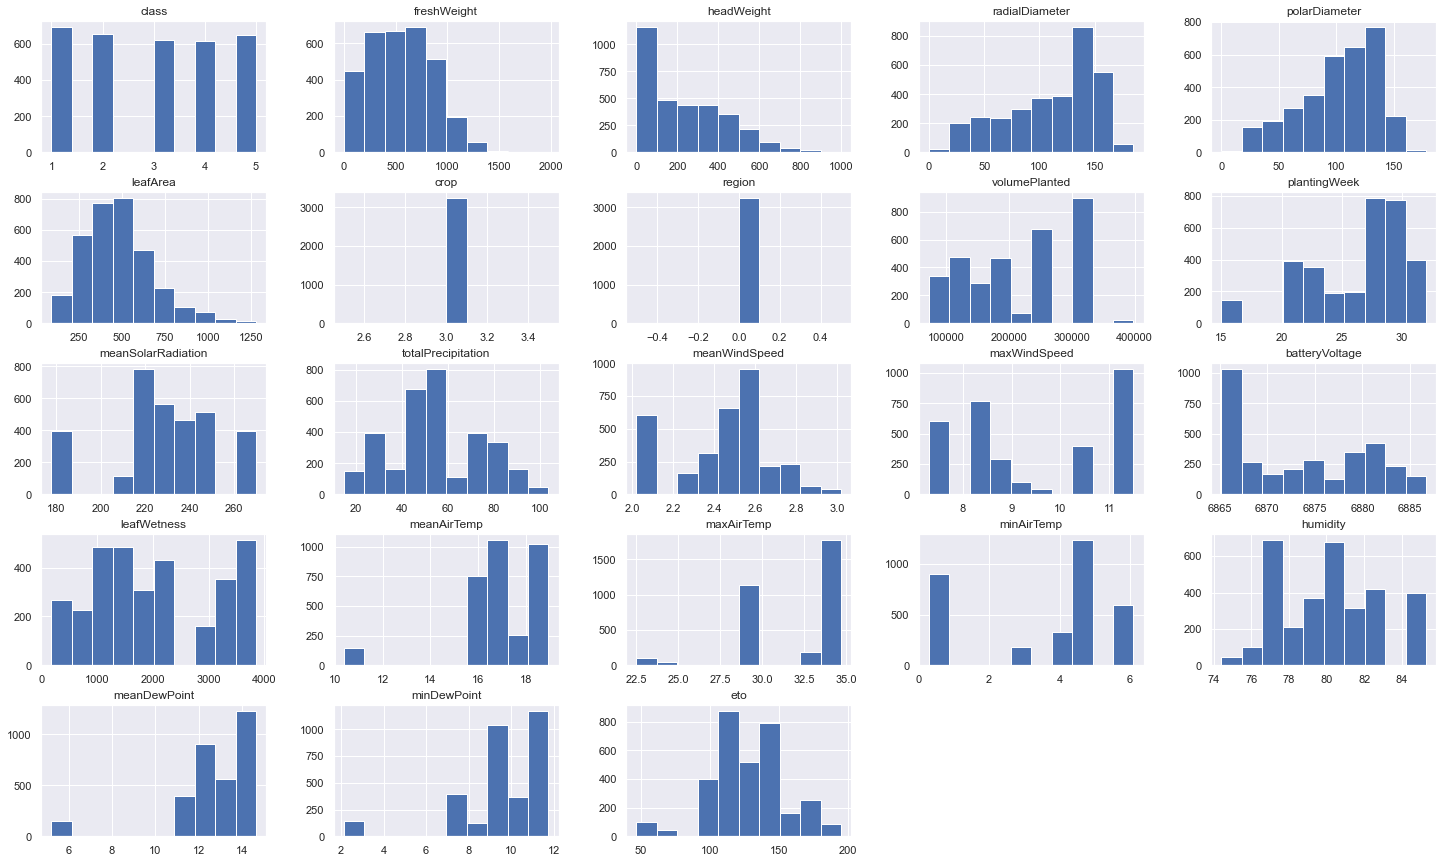
\includegraphics[width=\textwidth]{hist.png}
    \caption{Histograms of all the features}
    \label{figure:1}
\end{figure}

Finally we were left with the \emph{Weather} sheet. For us to be able to use information from this sheet in
the main DataFrame we were building, we implemented two functions. The first one returned a Series with an
average of the weather conditions a plant went through between two given dates. The second function also returned
a Series with weather information, but with data from the previous year. For the initial model testing we will
encode in the DataFrame information from the weather between \emph{Plant Date} and \emph{Flight Date} to predict
the final size of the crop at \emph{Check Date}. Depending on the result we may change this weather information
to get the weather conditions between \emph{Plant Date} and \emph{Check Date} from the previous year, also
with the possibility to retrieve information from more than one year in the past.

After the processing of the data, we analyzed the distribution of the data through a Histogram, illustrated
in Figure \ref*{figure:1}.

\section{Methodology}

After analyzing the data proided, we have identified that a multi-label linear regressor will probably allow
us to construct a useful model. Specifically, we plan to use the \emph{MultiOutputRegressor} class from
the \emph{ScikitLearn} library, which allows us to use any regressor as a multi-label regressor. First we
will implement Linear Regression, with the possibility to later on implement Decision Tree Regressor.

For training the model, we will use the \emph{ScikitLearn} tools to split our data into training and validation,
using a 70\% split for training and 30\% for validation. Being a regression problem, we will use Mean Squared Error
(MSE) to measure the error during the training phase, while using the Root Mean Squared Error (RMSE) to measure
the performance during the valudation phase.

\section{Conclusions}
While the weather is never the same, we believe it will be a useful feature to help us correctly estimate
the size of the crops for better planning for both the farmers and the supermarkets. After processing the data
we are confident that a useful model will be trainned and perform well. The team is open to testing other
Machine Learning tools and algorithms and deleting features that turn out not to be useful.

\bibliographystyle{abbrv}
\bibliography{sample}

\end{document}